\documentclass[10pt,a4paper]{article}
\usepackage[T1]{fontenc}
\usepackage[utf8]{inputenc}
\usepackage{lmodern}
\usepackage[margin=21mm]{geometry}
\usepackage{amsmath,amssymb,booktabs,longtable,tabularx,graphicx,hyperref,fancyhdr,enumitem,xcolor}
\definecolor{ink}{HTML}{21364D}
\hypersetup{colorlinks=true,urlcolor=ink,linkcolor=ink}
\setlength{\parindent}{0pt}\setlength{\parskip}{.50em}
\setlength{\emergencystretch}{3em}
\pagestyle{fancy}\fancyhf{}
\fancyhead[L]{\small PCM / ADMM tune-1 validation}
\fancyhead[R]{\small 9 November 2026}
\fancyfoot[C]{\thepage}
\setlength{\headheight}{14pt}
\begin{document}
{\LARGE\bfseries\color{ink} PnP-ADMM Tune-1: completed parameter search}\\[5pt]
{\large PCM at 20\% sampling with fixed NPL-default noise}\\[4pt]
{\color{gray} Experiment results report, version 1.0 | 9 November 2026}\\[4pt]
\textbf{Status: ADMM calibration complete (25/25); GS-PnP tuning and test set 45 pending.}
\par\medskip\hrule

\section{Executive summary}

We completed \textbf{25 independent Tune-1 calibration searches} for
PnP-ADMM-DRUNet, with five randomly selected validation acquisitions
from each of five PCM categories. All acquisitions used the original
20\% Hadamard sampling masks and NPL-default noise observations.
The hyperparameters were selected using held-out acquired measurements
without access to ground-truth images or test image metrics.

The search evaluated \textbf{420 distinct parameter configurations},
each using four fixed SSDU folds, for \textbf{1,680 fold reconstructions}.
All 25 selections are frozen. There were \textbf{zero failed candidates}.
The mean of the 25 individually selected SSDU prediction errors was
\textbf{0.004314767} (sample SD 0.000509679).

\textbf{Scope:} This report concerns \emph{validation-only tuning}.
The new configurations have not yet been evaluated on test set 45,
because the agreed test runner requires the 25 GS-PnP selections to be
frozen too. We therefore do not claim test PSNR, SSIM, HaarPSI or
reconstruction superiority from these calibration losses.

\section{Tuning algorithm}

For one calibration acquisition $y=Ax+\varepsilon$ at
$256\times256$ resolution and 20\% multilevel Hadamard sampling
($J=8$, coarse order $J_c=6$), the 13,107 acquired measurements
are split into four fixed SSDU folds. All 4,096 coarse rows remain
in the fit set; the remaining 9,011 acquired fine rows provide
held-out measurement subsets $\Lambda_k$.

For parameter vector $\theta=(\rho,\sigma)$, we minimise
\[
L(\theta)=\frac14\sum_{k=1}^{4}
\frac{\|A_{\Lambda_k}\widehat x_\theta(A_{\Theta_k},y_{\Theta_k})
-y_{\Lambda_k}\|_2^2}{|\Lambda_k|},
\]
where the reconstruction only sees the complementary rows $\Theta_k$.
The denoiser weights and ADMM solver remain fixed.

Search in logarithmic coordinates with positive parameter bounds
\[
\rho\in[0.03,4.0],\qquad \sigma\in[0.015,0.18].
\]
Start at the geometric midpoint. For each coordinate, evaluate two
interior points that divide its log interval into thirds, keeping the
two-thirds interval favoured by the lower SSDU loss.
Run \textbf{three contractions per coordinate and two coordinate
passes with reversed order}, caching duplicate evaluations.
Select the lowest \emph{actually evaluated} finite SSDU risk.

This approach assumes \emph{one-dimensional unimodality} of the
objective while other parameters are fixed. That assumption has
not been proved. It does not establish global optimality of
the nonlinear joint PnP objective.

\section{Step-by-step plan and execution}

\begin{enumerate}[leftmargin=1.5em]
\item Freeze the validation calibration sample IDs, test45 sample IDs,
RNG seed, archived acquisition SHA256 hashes, and parameter bounds.
\textbf{Complete}.
\item Verify the old normalised PCM data-fidelity convention,
four-fold measurement scoring, deterministic GPU behaviour, and
numerical search implementation. \textbf{Complete}.
\item Run five independent ADMM parameter searches per category.
Save candidate scores, original source checksums, fold diagnostics
and numerical errors. \textbf{Complete, 25 of 25}.
\item Freeze each winner as an independent validation-only
configuration. \textbf{Complete, 25 of 25}.
\item Run the separate GS-PnP calibration searches. \textbf{Pending,
deliberately not started}.
\item When all 50 selections are frozen, reconstruct the fixed
test set 45, nine images per category, using all acquired rows.
\textbf{Pending}.
\item Compare with existing PCM methods using image
PSNR, SSIM, HaarPSI, MSE, runtimes, and stored reconstruction
arrays. \textbf{Pending}.
\end{enumerate}

\section{Experiment running and numerical checks}

The ADMM search used \textbf{tuni's NVIDIA RTX 4070}, with
deterministic CUDA/CuDNN settings and the original DRUNet weights.
Each candidate requires four complete ADMM reconstructions, with
the original maximum of 100 iterations and residual-based stopping.
Candidate caching reduced the realised search from the maximum of
25 evaluations per calibration to a mean of
\textbf{16.8}, with range 13--19.
Each complete SSDU fold reconstruction took a mean of
1.253 seconds in the archived execution records,
but timing varies with the chosen parameter and stopping behaviour.

Completed: 25 calibrations, 420 candidates, 1,680 fold
reconstructions. No invalid candidates were recorded.
The frozen selections and every scored fold remain on tuni.
\emph{The RTX 4070 was not used to evaluate test45 reconstruction
quality in this phase.}

\section{Results and deliverables}

\subsection*{Five PCM category summaries}

\begin{table}[htbp]
\centering\small
\begin{tabular}{@{}lrrrrr@{}}
\toprule
Category & Mean SSDU & SD SSDU & Median $\rho$ & Median $\sigma$ & Mean probes\\
\midrule
CIGS & 0.00372777 & 0.00009815 & 0.78297 & 0.05196 & 15.2 \\
Organic & 0.00435453 & 0.00013780 & 0.78297 & 0.07862 & 18.2 \\
Perovskite & 0.00404770 & 0.00045409 & 0.78297 & 0.05196 & 16.0 \\
Reference & 0.00462750 & 0.00052702 & 0.78297 & 0.05196 & 16.0 \\
Silicone & 0.00481633 & 0.00029584 & 0.37926 & 0.10362 & 18.6 \\
\bottomrule
\end{tabular}
\caption{Each category contains five independently tuned validation
measurements. Mean and sample SD describe selected held-out
\emph{measurement} MSE, not image reconstruction error.}
\end{table}

\subsection*{All 25 independently selected ADMM configurations}

\small
\begin{longtable}{@{}lrrrrr@{}}
\toprule
Category & Validation ID & $\rho$ & $\sigma$ &
SSDU MSE & Candidate evaluations\\
\midrule
\endfirsthead
\toprule
Category & Validation ID & $\rho$ & $\sigma$ &
SSDU MSE & Candidate evaluations\\
\midrule
\endhead
CIGS & 0008 & 1.93756 & 0.05196 & 0.00366939 & 13 \\
CIGS & 0530 & 0.45461 & 0.07862 & 0.00363170 & 19 \\
CIGS & 0589 & 0.78297 & 0.05196 & 0.00367037 & 13 \\
CIGS & 0733 & 0.78297 & 0.04962 & 0.00384259 & 18 \\
CIGS & 0768 & 0.78297 & 0.05196 & 0.00382482 & 13 \\
Organic & 0158 & 0.78297 & 0.05965 & 0.00422714 & 18 \\
Organic & 0530 & 0.45461 & 0.08620 & 0.00446876 & 18 \\
Organic & 0589 & 0.78297 & 0.07862 & 0.00452695 & 18 \\
Organic & 0733 & 0.45461 & 0.08620 & 0.00422868 & 19 \\
Organic & 0768 & 0.78297 & 0.07862 & 0.00432111 & 18 \\
Perovskite & 0008 & 0.78297 & 0.05196 & 0.00446728 & 13 \\
Perovskite & 0045 & 0.65320 & 0.05965 & 0.00461581 & 18 \\
Perovskite & 0733 & 0.93853 & 0.05965 & 0.00372562 & 18 \\
Perovskite & 0768 & 0.78297 & 0.04962 & 0.00369531 & 18 \\
Perovskite & 0917 & 0.78297 & 0.05196 & 0.00373448 & 13 \\
Reference & 0008 & 0.93853 & 0.05196 & 0.00523090 & 13 \\
Reference & 0045 & 0.45461 & 0.07171 & 0.00474304 & 18 \\
Reference & 0158 & 0.65320 & 0.05196 & 0.00499911 & 13 \\
Reference & 0396 & 0.78297 & 0.07862 & 0.00410190 & 18 \\
Reference & 0768 & 0.93853 & 0.04962 & 0.00406253 & 18 \\
Silicone & 0008 & 0.65320 & 0.12456 & 0.00526204 & 19 \\
Silicone & 0158 & 0.31640 & 0.07862 & 0.00483393 & 18 \\
Silicone & 0283 & 0.18371 & 0.12456 & 0.00479944 & 19 \\
Silicone & 0589 & 0.37926 & 0.10362 & 0.00443315 & 19 \\
Silicone & 0733 & 0.37926 & 0.10362 & 0.00475311 & 18 \\
\bottomrule
\end{longtable}
\normalsize

\begin{figure}[htbp]\centering
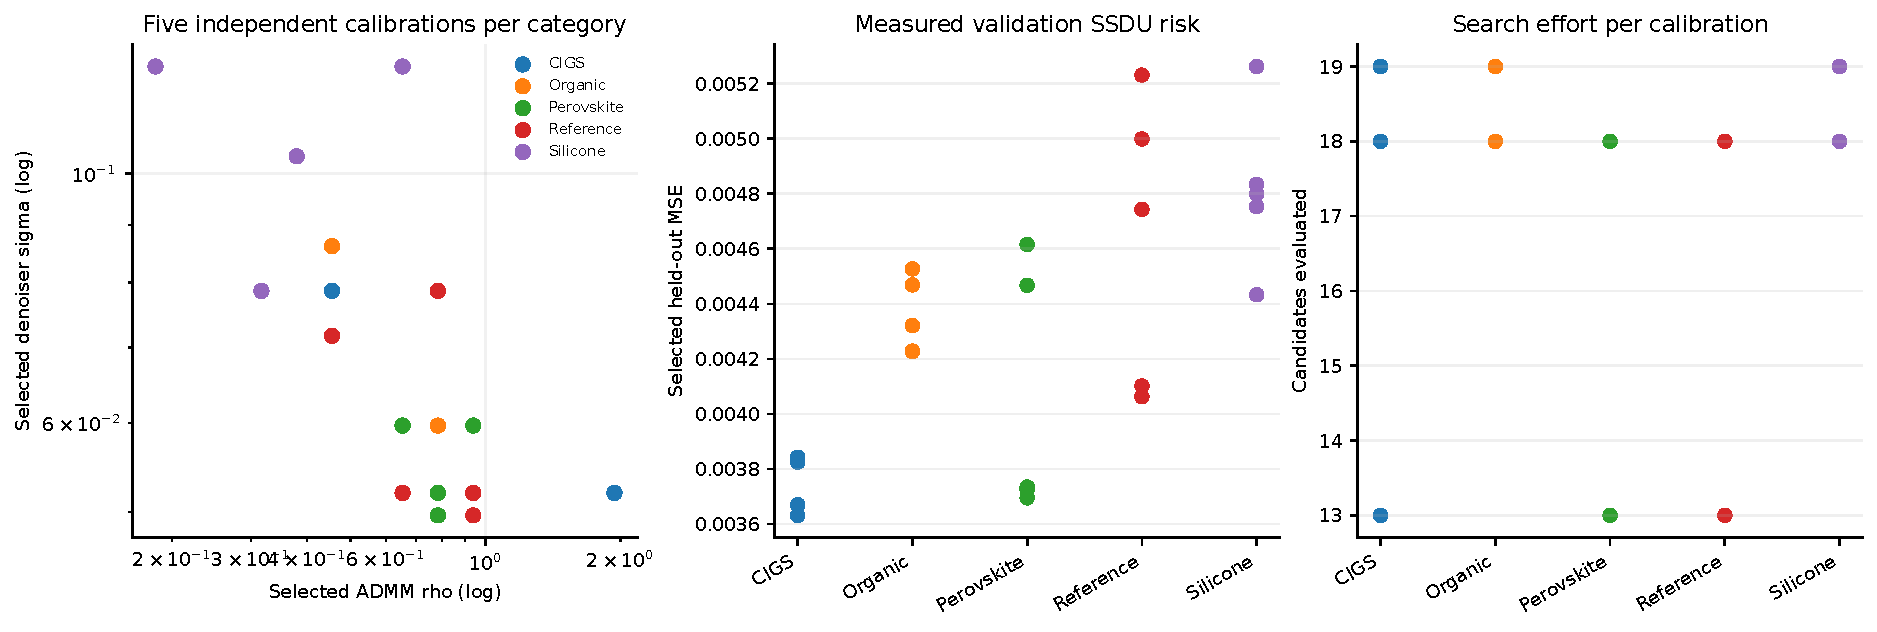
\includegraphics[width=.82\linewidth]{figures/admm_tune1_25_summary.pdf}
\caption{Selected regularisation/denoiser parameters,
per-calibration SSDU prediction loss and candidate evaluation counts.}
\end{figure}

\clearpage
\begin{figure}[htbp]\centering
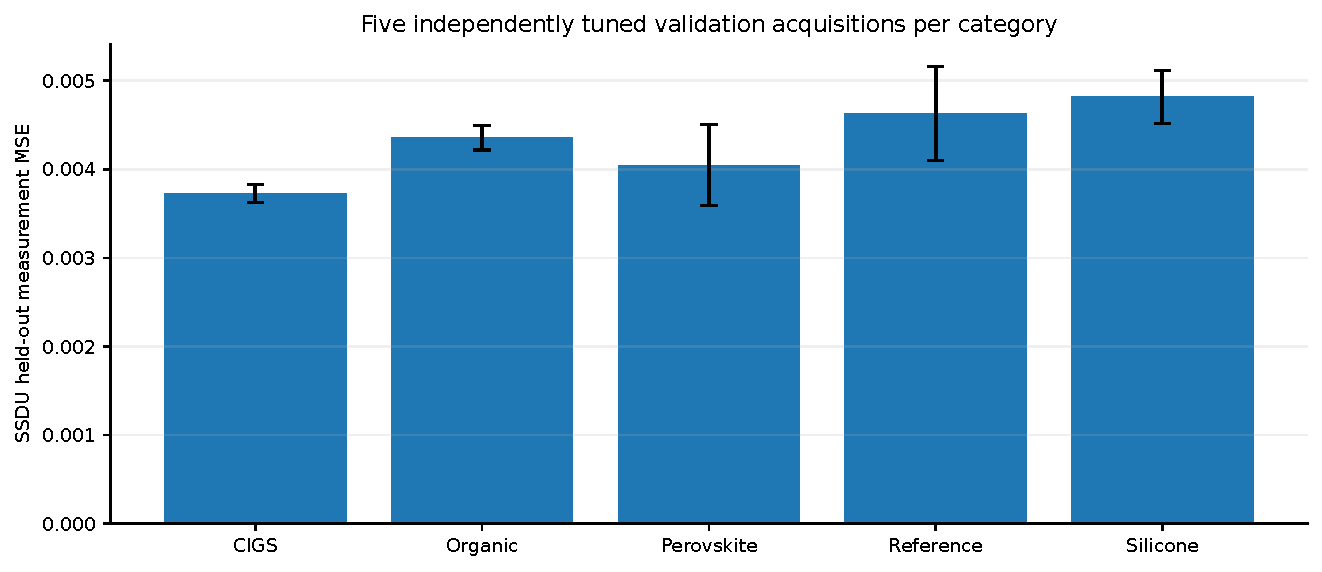
\includegraphics[width=.64\linewidth]{figures/admm_tune1_category_loss.pdf}
\caption{Within-category mean and sample SD of selected SSDU loss.}
\end{figure}

\subsection*{Reproducibility deliverables}

The ZIP contains the full 25-selection JSON/CSV summary, all 420
candidate JSON score files with four SSDU-fold records each,
all frozen parameter files and search traces, the fixed validation
and test45 manifests, source scripts, operator/scoring provenance,
and this editable \LaTeX{} report with its figures and PDF.
No test45 raw images or test quality metrics are included,
because no test45 run has been performed.

\section{Conclusion}

The category-wise Tune-1 parameter search for PnP-ADMM is
\textbf{complete and numerically successful}: all 25 independent
validation-only selections were frozen, with no recorded candidate
failure. The selected $\rho$ and denoiser $\sigma$ values vary
across calibration acquisitions, so a single universal parameter
pair is not established by this experiment.

A lower held-out measurement error does not necessarily imply
higher image PSNR or preservation of thin lines.
The next required study is transfer of each frozen configuration
to its nine category-matched test45 images, followed by
comparison with existing methods. GS-PnP calibration has been
left untouched as requested.

\paragraph{Primary references.}
Yaman et al. (2020), SSDU measurement partitioning,
\url{https://doi.org/10.1002/mrm.28378}.

Hurault, Leclaire and Papadakis (2022), gradient-step
plug-and-play with backtracking,
\url{https://openreview.net/pdf?id=fPhKeld3Okz}.
\end{document}
